\documentclass[a4paper, 11pt]{article}

\usepackage{vmargin}

\setmarginsrb{2cm}{1cm}{2cm}{1cm}{1cm}{2cm}{1cm}{2cm}
%1 est la marge gauche
%2 est la marge en haut
%3 est la marge droite
%4 est la marge en bas
%5 fixe la hauteur de l'entête
%6 fixe la distance entre l'entête et le texte
%7 fixe la hauteur du pied de page
%8 fixe la distance entre le texte et le pied de page
%------------------------------Packages généraux------------------------------

\usepackage[french]{babel}
\usepackage[T1]{fontenc}
\usepackage{ae}
\usepackage[utf8]{inputenc}

%------------------------------Mathématiques------------------------------

\usepackage{amsmath}
\usepackage{amssymb}
\usepackage{amsthm}
\usepackage{amsfonts}
\usepackage{eucal}


%------------------------------Graphics------------------------------

\usepackage{graphicx}
\usepackage{fancyhdr}
\usepackage{fancybox}
\usepackage{color}
\usepackage{epstopdf}
\usepackage{float}
\usepackage{slashbox}
%------------------------------Syntaxe------------------------------

\usepackage{listings}
\lstloadlanguages{Matlab}

\def\refmark#1{\hbox{$^{\ref{#1}}$}}
\DeclareSymbolFont{cmmathcal}{OMS}{cmsy}{m}{n} %Mathcal correcte
\DeclareSymbolFontAlphabet{\mathcal}{cmmathcal}
\renewcommand\thesubsection{\alph{subsection}}


%------------------------------Inclure code MatLab------------------------------

\usepackage{listings}
\newcommand*\styleC{\fontsize{9}{10pt}\usefont{T1}{ptm}{m}{n}\selectfont }
\newcommand*\styleD{\fontsize{9}{10pt}\usefont{OT1}{pag}{m}{n}\selectfont }

\makeatletter
% on fixe le langage utilisé
\lstset{language=matlab}
\edef\Motscle{emph={\lst@keywords}}
\expandafter\lstset\expandafter{%
  \Motscle}
\makeatother


\definecolor{Ggris}{rgb}{0.45,0.48,0.45}

\lstset{emphstyle=\rmfamily\color{blue}, % les mots réservés de matlab en bleu
basicstyle=\styleC,
keywordstyle=\ttfamily,
commentstyle=\color{Ggris}\styleD, % commentaire en gris
numberstyle=\tiny\color{red},
numbers=left,
numbersep=10pt,
lineskip=0.7pt,
showstringspaces=false}
%  % inclure le fichier source
\newcommand{\FSource}[1]{%
\lstinputlisting[texcl=true]{#1}
}

\usepackage[section]{placeins}

\let\cleardoublepage\clearpage

%------------------------------Début du document------------------------------

\begin{document}
%------------------------------Page de garde------------------------------

\begin{titlepage}
	
	
	\begin{tabular}{p{11cm}p{8cm}}    
		\includegraphics[scale=0.4]{Fig/logo_ulg.png}  &\raggedright{\includegraphics[scale=0.6]{Fig/Logo_FSAnew.png}}\\
	\end{tabular}
	
	\begin{center}
		\unitlength = 1cm
		\vspace{0.1cm}
		\Large\textbf{Faculté des sciences appliquées}\\
		\vspace{2.5cm}
		\Large  \bsc{MATH0487-2\\Eléments de statistique\\}
		\vspace*{2cm}
		\bsc{Partie 1 du projet personnel}
		\huge
		\begin{center}
			Projet 2\\
			\rule{13cm}{0.5mm}
		\end{center}
	\end{center}
	
	\vspace*{4cm}
	
	\centering{\large \noindent  \it Antoine \bsc{Wehenkel}}
	\vspace*{4cm}
	
	
	\begin{tabular}{p{14cm}p{15cm} l r}    
		Année académique 2015-2016 
		&\raggedright{\large \noindent \textsl{22 octobre 2015}}
	\end{tabular}
\end{titlepage}
% -------- Fin Page de garde --------
   \setcounter{page}{1}
   \section{Analyse descriptive}
   \subsection{Histogramme des résultats aux questions de théorie}
   \begin{figure} [H]
	\begin{center}
		\includegraphics[height=6cm, width = 5.5cm]{Fig/Q1A1.eps}
		\includegraphics[height=6cm, width = 5.5cm]{Fig/Q1A2.eps}
		\includegraphics[height=6cm, width = 5.5cm]{Fig/Q1A3.eps}
		\caption{Histogrammes des questions de théories}
		\label{Q1A}
	\end{center}	
	\end{figure}
 Les trois histogrammes représentants les résultats aux questions de théorie sont présentés à la \bsc{figure} \ref{Q1A}. Ces histogrammes ont été réalisés à l'aide des résultats d'une population de 147 étudiants. On observe que la première question a été bien faite par les étudiants. La cote la plus répandue(le mode) est \bsc{17}(21 étudiants), de manière globale plus une note s'éloigne de cette valeur moins le nombre d'étudiants l'ayant obtenue est important. Du second histogramme il ne resort pas de véritable tendance générale, la note la plus obtenue(le mode) est 11 mais seulement 13 étudiants l'ont obtenus. Cette question a été réussie par environ la moitié des étudiants. Pour la troisième question on observe que le mode vaut 0(plus de 30 étudiants). Une grande majorité des étudiants a obtenu moins de la moitié pour cette question. En comparant les trois histogrammes on voit directement que la question 1 est la mieux faite, que la troisième est la plus ratée et que la seconde se situe entre ces deux situations.
 	\subsection{Caractéristiques des résultats aux exercices}
 	\begin{figure}[H]
 	\begin{center}
   			\begin{tabular}{|l|l|l|l|l|}
				\hline
				 \backslashbox{Valeurs}{Question} & 1 & 2 & 3 \\
				\hline
				Moyenne & 7,9388  &  16,3946  &  8,6735  \\
  				Médiane & 8  &  18  &  8  \\
  				Mode & 8  &  18  &  6  \\
   				Ecart-type & 3,7475  &  4,1887  &  4,6220  \\
				\hline
			\end{tabular}
			\caption{Valeurs caracterisants les résultats aux exercices} \label{Q1B}
		\end{center}
		\end{figure}
En comparant les résultats on voit que l'exercice 2 a la note moyenne la plus élevée(environ 16,5) les deux autres exercices ont été  moins faits bien avec pour les deux une note moyenne proche de 8. La médiane du second exercice vaut 18, 18 est également le mode pour cette question celà veut dire que 18 est la note la plus donnée aux étudiants et en plus qu'il y a autant d'étudiants ayant une note supérieure à 18 que d'étudiants ayant moins de 18. Pour le premier exercice la médiane est égale au mode et quasi égale à la moyenne, l'écart type de cette question est le plus faible. On peut conclure de celà que cette question est celle où le plus d'étudiants ont obtenus des cotes proches les unes des autres. Les écarts type des question 2 et 3 sont plus élevées et donc les notes varient plus les unes par rapport aux autres. La \bsc{figure} \ref{Q1B} reprend tous ces résultats de manière précise et organisée.\\
On définit un résultat normal s'il est compris dans l'intervalle \bsc{[moyenne - écart-type; moyenne + écart-type]} ces résultats sont rassemblés sur la \bsc{figure} \ref{Q1B2}. On observe que l'exercice 2 a le plus grand pourcentage de résultats normaux.
\begin{figure}[H]
 	\begin{center}
   			\begin{tabular}{|l|l|l|l|l|}
				\hline
				  & Exercice 1 & Exercice 2 & Exercice 3 \\
				\hline
				Borne inférieure & 4,1913 &  12,2059  &  4,0515  \\
  				Borne supérieure & 11,6863 &  20,5832  & 13,2955  \\
  				Proportion d'étudiants dans l'intervalle & 0,6190   & 0,8776  &  0,6803\\
				\hline
			\end{tabular}
			\caption{Résultats "normaux"} \label{Q1B2}
		\end{center}
		\end{figure}
   \subsection{Boites à moustache des résultats aux projets}
   \begin{figure} [H]
	\begin{center}
		\includegraphics[height=6cm, width = 7cm]{Fig/Q1C1.eps}
		\includegraphics[height=6cm, width = 7cm]{Fig/Q1C2.eps}
		\includegraphics[height=6cm, width = 7cm]{Fig/Q1C3.eps}
		\caption{Boites à moustache des résultats aux projets}
		\label{Q1C}
	\end{center}	
	\end{figure}
	On remarque immédiatemment sur la \bsc{figure} \ref{Q1C} qu'il y a un certain nombre de données abérrantes pour les notes des deux projets et que par contre à la question d'examen portant sur le projet deux il n'y a pas de donnée aberrante. Les quartiles ont les valeurs données à la \bsc{figure} \ref{Q1C2}. Une remarque sur le troisième quartile de la Q2 c'est que la valeur est à virgule cependant les chiffres après la virgule sont choisis de manière arbitraire(ici c'est la fonction quantil de matlab qui a décidé) ils n'ont pas de signification réelle.
	\begin{figure}[H]
 	\begin{center}
   			\begin{tabular}{|l|l|l|l|l|}
				\hline
				  & Projet 1 & Projet 2 & Question sur le projet 2 \\
				\hline
				Q1 & 15  &  17  &   4  \\
  				Médiane & 16  &  18  &   8  \\
  				Q2 & 18  & 19  & 12,75\\
				\hline
			\end{tabular}
			\caption{Résultats "normaux"} \label{Q1C2}
		\end{center}
		\end{figure}
\subsection{Définition de deux nouvelles variables}
Les deux nouvelles variables sont les moyennes de chaque étudiant aux exercices et à la théorie, elles sont créées en additionnant leurs trois résultat dans chacun des domaines et en divisant cette somme par 3. Leur polygone respectif de fréquences cumulées est présenté à la \bsc{figure}\ref{Q1D}. Le pourcentage d'élèves ayant entre 10 et 14 aux questions de théorie est environ de 34\%, pour les exercices le pourcentage est d'environ 57,8\%. Ces valeurs peuvent être obtenues à l'aide du graphique, il suffit de faire la différence des valeurs du polygone en 14 et en 10.
   \begin{figure} [H]
	\begin{center}
		\includegraphics[height=6cm, width = 7cm]{Fig/Q1D1.eps}
		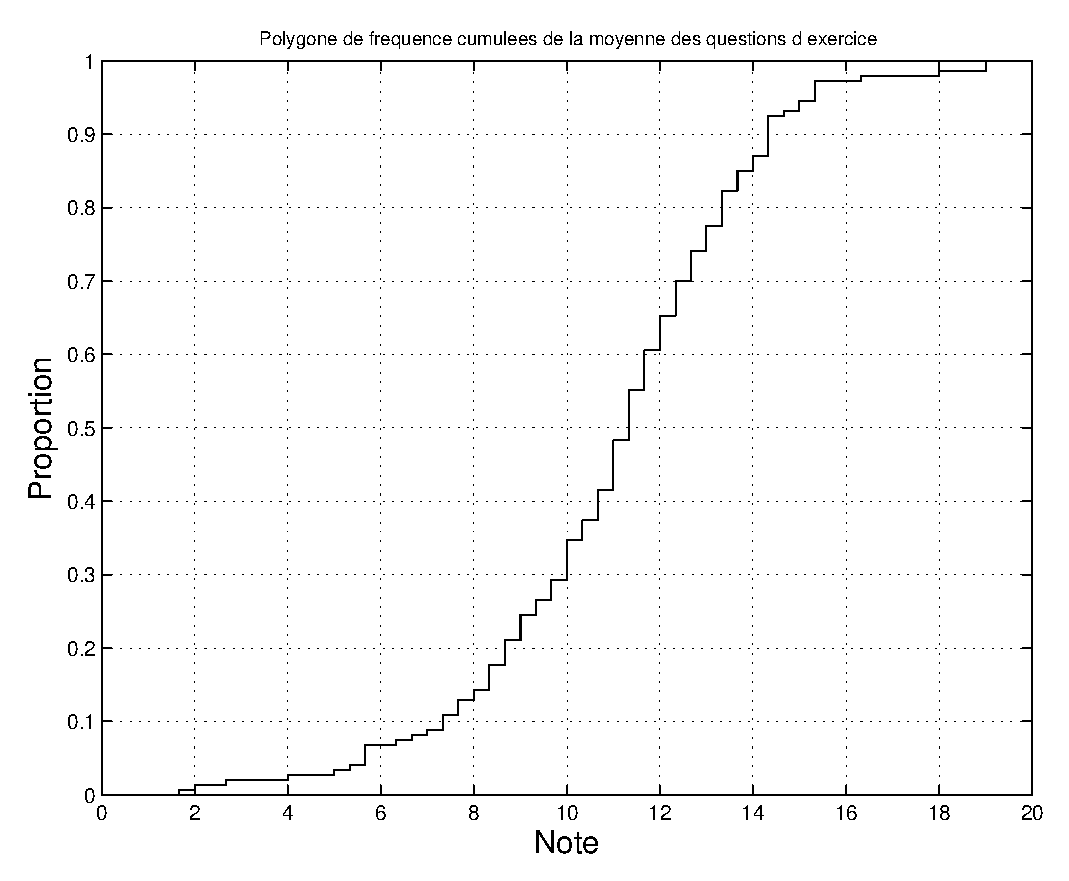
\includegraphics[height=6cm, width = 7cm]{Fig/Q1D2.eps}
		\caption{Polygones de fréquences cumulées des deux nouvelles variables}
		\label{Q1D}
	\end{center}	
	\end{figure}
\subsection{Scatterplot projet 2 et question portant dessus}
\begin{figure} [H]
	\begin{center}
		\includegraphics[height=9cm, width = 16cm]{Fig/Q1E.eps}
				\caption{Scatterplot}
		\label{Q1E}
	\end{center}
\end{figure}
Le coefficient de corrélation vaut 0,1128. Ces deux variables ne sont pas fortement correlées. On peut seulement dire que pour réussir la question sur le projet il fallait avoir réussi le projet.
   \section{Génération d'échantillon i.i.d}
   \subsection{Echantillon de 20 étudiants}
   \paragraph{Moyenne, médiane, écart-type des exercices}
   	\begin{figure}[H]
 	\begin{center}
   			\begin{tabular}{|l|l|l|l|l|}
				\hline
				  & Exercice 1 & Exercice 2 & Exercice 3 \\
				\hline
				Moyenne échantillon & 6,85  &  16,35  &   9,2  \\
  				Moyenne population & 7,9388  &  16,3946  &  8,6735  \\
  				\hline
  				Médiane échantillon & 6  & 18  & 9\\
  				Médiane population & 8  &  18  &  8  \\
  				\hline
  				Ecart-type échantillon & 3,7480  & 4,6573  & 2,6907\\
  				Ecart-type population & 3,7475  &  4,1887  &  4,6220  \\
				\hline
			\end{tabular}
			\caption{Caracteristiques échantillon} \label{Q2a1}
		\end{center}
		\end{figure}
		Les différentes valeurs de l'échantillon s'approchent assez bien des valeurs de la population cependant un échantillon de 20 étudiants ne suffit pas à représenter de manière précise la population. En effet les valeurs de la moyenne s'éloignent jusqu'à 1,1 points de la vraie valeur. Pour la médiane c'est 2 points. Et pour l'écart type il s'éloigne de presque 2 points dans le pire cas.
	\paragraph{Boîte à moustache des résultats portant sur les projets}
	   \begin{figure} [H]
	\begin{center}
		\includegraphics[height=6cm, width = 7cm]{Fig/Q2A21.eps}
		\includegraphics[height=6cm, width = 7cm]{Fig/Q2A22.eps}
		\includegraphics[height=6cm, width = 9cm]{Fig/Q2A23.eps}
		\caption{Boites à moustache des résultats aux projets}
		\label{QA2}
	\end{center}	
	\end{figure}
	On observe que les boîtes à moustache ont des allures similaires à celles de la population cependant en y regardant de plus prêt on voit de grosses différences dans les valeurs des quartiles. Un échantillon ne suffit pas à représenter de manière précise la population.
	\paragraph{Polygone de fréquences cumulées et distance de Kolmogorov Smirnov pour les questions de théorie} 
	\begin{figure} [H]
	\begin{center}
		\includegraphics[height=6cm, width = 12cm]{Fig/Q2A3.eps}
		\caption{Polygone de fréquences cumulées}
		\label{Q2A3}
	\end{center}	
	\end{figure}
	La distance de Kolmogorov Smirnov entre les deux polygones vaut 0,1847. Le polygone de l'échantillon est assez éloigné de celui de la population, celà est du en grande partie au fait que les premier à un caractère beaucoup plus discret car le nombre de points est bien plus faible que pour tracer le polygone de la population.
	\subsection{100 échantillons de 20 étudiants}
\paragraph{Moyennes de l'exercice 1} 
	\begin{figure} [H]
	\begin{center}
		\includegraphics[height=6cm, width = 12cm]{Fig/Q2B1.eps}
		\caption{Histogramme des moyennes de l'exercice 1}
		\label{Q2B}
	\end{center}	
	\end{figure}
	On peut vaguement reconnaitre une loi normale sur l'histogramme avec une valeur centrale(la moyenne pour une loi normale) un peu en dessous de 8. Si l'on teste le code avec un plus grand nombre d'échantillon la loi normale se marque plus précisement. On obtient 7,9860 comme moyenne des valeurs moyennes. La moyenne de la population étant 7,9388 on en est relativement proche, bien plus qu'avec un échantillon unique.
\paragraph{Médianes de l'exercice 1} 
	\begin{figure} [H]
	\begin{center}
		\includegraphics[height=6cm, width = 12cm]{Fig/Q2B2.eps}
		\caption{Histogramme des médianes de l'exercice 1}
		\label{Q2B}
	\end{center}	
	\end{figure}
	On peut vaguement reconnaitre une loi normale sur l'histogramme avec une valeur centrale(la moyenne pour une loi normale) prenant la valeur 8. Il serait cependant impossible d'obtenir une distribution réellement normale étant donné que la médiane prend un nombre fini de valeur alors que la loi normale est une loi continue. On obtient 8,0250 comme moyenne des médianes cette valeur est moins proche de la moyenne de la population que la moyenne des moyennes.
	\paragraph{Ecarts-types de l'exercice 1} 
	\begin{figure} [H]
	\begin{center}
		\includegraphics[height=6cm, width = 12cm]{Fig/Q2B3.eps}
		\caption{Histogramme des écarts-type obtenus à l'exercice 1}
		\label{Q2B}
	\end{center}	
	\end{figure}
	Ici on ne reconnait pas de loi connue. La valeur moyenne des écarts-types vaut 3,4906 alors que l'écart-type de la population vaut 3,7475. Ces valeurs ne sont pas très proches. Pour approcher mieux le vrai écart type il faudrait prendre la racine de la variance corrigée.
	\paragraph{Distance de Kolmogorov Smirnov concernant l'exercice 1} 
   \begin{figure} [H]
	\begin{center}
		\includegraphics[height=6cm, width = 7cm]{Fig/Q2B4.eps}
		\includegraphics[height=6cm, width = 7cm]{Fig/Q2B5.eps}
		\includegraphics[height=6cm, width = 7cm]{Fig/Q2B6.eps}
		\caption{Distance de Kolmogorov Smirnov pour les 3 exercices}
		\label{Q2B3}
	\end{center}	
	\end{figure}
	On observe que les trois histogrammes ont la même allure, en effet la théorie nous dit:\textit{ "la distribution d’échantillonnage de DKS
n,X ne dépend en fait pas de l’allure de FX , pour autant que FX soit continue."} 
\newpage
\appendix
\section{Q1A}
\lstset{breaklines=true}
\lstset{
   literate={ö}{{\"o}}1
            {ô}{{\^o}}1
            {î}{{\^i}}1
            {ï}{{\"o}}1
            {ç}{{\,c}}1
            {à}{{\`a}}1
            {â}{{\^a}}1
            {ä}{{\"a}}1
            {é}{{\'e}}1
            {è}{{\`e}}1
            {ê}{{\^e}}1
            {ë}{{\"e}}1
            {û}{{\^u}}1
            {ü}{{\"u}}1
 }
\lstinputlisting[language=matlab]{code/Q1A.m}
\section{Q1B}
\lstinputlisting[language=matlab]{code/Q1B.m}
\section{Q1C}
\lstinputlisting[language=matlab]{code/Q1C.m}
\section{Q1D}
\lstinputlisting[language=matlab]{code/Q1D.m}
\section{Q1E}
\lstinputlisting[language=matlab]{code/Q1E.m}
\section{Q2A}
\lstinputlisting[language=matlab]{code/Q2A.m}
\section{Q2B}
\lstinputlisting[language=matlab]{code/Q2B.m}

\end{document}